\documentclass[12pt, a4paper]{article}

%###################################################################
% PACKAGES
%###################################################################

    \usepackage[utf8]{inputenc}

    \usepackage[T1]{fontenc}

    \usepackage{lmodern}

    \usepackage{amsmath, amssymb}

    \usepackage{graphicx}

    \usepackage{float}

    \usepackage{enumitem}

    \usepackage{longtable}

    \usepackage{array}

    \usepackage[ngerman]{babel}

    % \usepackage[backend=biber,style=numeric]{biblatex}
    \usepackage{glossaries}
    
    \usepackage{geometry}

    \usepackage{xcolor}
    
    \usepackage{listings}

    \usepackage{fancyhdr}

    \usepackage{siunitx}

    \usepackage{hyperref}



% ###################################################################
% PREAMBLE
% ###################################################################

\hypersetup{
    colorlinks=true,
    linkcolor=blue,
    filecolor=magenta,      
    urlcolor=cyan,
    pdftitle={Overleaf Example},
    pdfpagemode=FullScreen,
}

 \geometry{
    a4paper,
    left=30mm,
    top=30mm,
 }

\setlength{\headheight}{14.49998pt}

\pagestyle{fancy}

\fancyhead{}

\fancyhead[L]{\thepage}

\title{Simultationstechnik -\\
    Programmentwurf}

\author{Carl Galman (4958469) \\
    Jonas Fischer (9836182) \\
    Jonas Zeller (7079186) }



\date{\today}



% ###################################################################
% DOCUMENT
% ###################################################################

\begin{document}

    \maketitle


    \newpage

    \tableofcontents

    \newpage

    \listoffigures

    \newpage

    \section*{Einleitung }
    
In dieser Arbeit wird ein Einspurmodell zur Beschreibung der lateralen Fahrzeugdynamik
untersucht. Grundlage der Analyse sind sowohl ein nichtlineares als auch ein linearisiertes
Modell, welche in Simulink umgesetzt wurden.

Der Arbeit liegen zwei Simulink-Dateien bei. Die erste Datei enthält sowohl das
nichtlineare als auch das linearisierte Einspurmodell. Diese wurde für die Aufgaben~2 und~3
verwendet, in denen die Modellgleichungen implementiert sowie das Verhalten des linearen
und des nichtlinearen Systems miteinander verglichen wird.

Die zweite Simulink-Datei enthält ausschließlich das linearisierte Modell und wurde für die
Untersuchung des Frequenzverhaltens in den Aufgaben~4 und~5 verwendet, insbesondere für die
Bestimmung des Frequenzgangs und die Darstellung der Bodediagramme.

Zusätzlich ist ein MATLAB-Live-Skript beigefügt, in dem die Aufgaben~1, 4 und~5 bearbeitet
wurden. Darin sind die analytischen Berechnungen sowie die Auswertung der Simulationen
und Frequenzgänge umgesetzt.

Die Grundlage des verwendeten Modells bilden die folgenden nichtlinearen Differentialgleichungen
des Einspurmodells, wie sie in der Aufgabenstellung gegeben sind. Diese beschreiben die
Schräglaufwinkel der Reifen sowie die Dynamik des Schwimmwinkels $\beta$ und der Gierrate
$\dot{\Psi}$.

\subsection*{Nichtlineare Modellgleichungen}

Dynamik des Schwimmwinkels:
\begin{equation}
\dot{\beta}
=
-\dot{\Psi}
+
\frac{1}{m v}
\left(
c_v \alpha_v \frac{\cos(\delta)}{\cos(\beta)}
+
c_h \alpha_h \frac{1}{\cos(\beta)}
\right)
\label{eq:betadot}
\end{equation}
\\
Dynamik der Gierrate:
\begin{equation}
\ddot{\Psi}
=
\frac{1}{J}
\left(
l_v c_v \alpha_v \cos(\delta)
-
l_h c_h \alpha_h
\right)
\label{eq:psiddot}
\end{equation}
\\
Schräglaufwinkel an der Vorderachse:
\begin{equation}
\alpha_v
=
\delta
-
\frac{l_v \dot{\Psi}}{v \cos(\beta)}
+
\tan(\beta)
\label{eq:alphav}
\end{equation}
\\
Schräglaufwinkel an der Hinterachse:
\begin{equation}
\alpha_h
=
\frac{l_h \dot{\Psi}}{v \cos(\beta)}
-
\tan(\beta)
\label{eq:alphah}
\end{equation}
\\
Dabei bezeichnet $m$ die Fahrzeugmasse, $v$ die Fahrzeuggeschwindigkeit,
$J$ das Trägheitsmoment um die Hochachse, $l_v$ und $l_h$ die Abstände des
Schwerpunkts zu Vorder- bzw. Hinterachse sowie $c_v$ und $c_h$ die
Reifensteifigkeiten der Vorder- und Hinterachse.
    \newpage
    \section{Aufgabe 1}
    \subsection{Zustandsvekotrepresentation}

In diesem System sind zwei Gleichungen gegebn, die 
die Dynamik des Systems beschreiben. 

Die erste Gleichung beschreibt die Änderung der Gierwinkelgeschwindigkeit $\dot{\psi}$ und die zweite Gleichung beschreibt die Änderung des Seitenwindwinkels $\beta$.
Somit haben wir zwei Zustandsgrößen, die wir in einem Zustandsvektor $Y$ zusammenfassen können, da die beide erste Ordnung in Abhängigkeit von 
$\beta \text{und} \dot{\psi}$ sind,
folgt somit die folgende Zustandsvektorrepresentation:


\begin{equation}  
Y = 
    \begin{bmatrix}
        \beta \\
        \dot{\psi}
    \end{bmatrix}
    \quad \Rightarrow \quad
    \dot{Y} = 
    \begin{bmatrix}
        \dot{\beta} \\
        \ddot{\psi}
    \end{bmatrix} =
    \begin{bmatrix}
        -\dot{\psi} + \frac{1}{m\cdot v} \cdot (c_v \alpha_v(\beta) \frac{\cos(\delta)}{\cos(\beta)}+ c_h \alpha_h(\beta) \frac{1}{\cos(\beta)}) \\
        \frac{1}{J} \cdot (c_v \alpha_v(\beta) l_v \cos(\delta) + c_h \alpha_h(\beta) l_h)
    \end{bmatrix}
\end{equation}

mit den Funktionen $\alpha_v(\beta)$ und $\alpha_h(\beta)$ der Schräglaufwinkeln, die wie folgt definiert sind:

\begin{equation}
    \alpha_v(\beta) = \delta - \frac{l_v\cdot \dot{\psi}}{v\cdot \cos(\beta)} + \tan{\beta} 
\end{equation}
\begin{equation}
    \alpha_h(\beta) = - \frac{l_h\cdot \dot{\psi}}{v\cdot \cos(\beta)} - \tan{\beta}
\end{equation}

\subsection{Solverauswahl}

Die Dynamik des Systems ist nichtlinear, da die Funktionen $\alpha_v(\beta)$ und $\alpha_h(\beta)$ nichtlinear in Bezug auf $\beta$ und $\dot{\psi}$ sind.
Die Dynamik des Systems wird auch explizit als glattes System beschrieben, da die Funktionen $\alpha_v(\beta)$ und $\alpha_h(\beta)$ stetig differenzierbar sind.

Nach der Analyse der Dynamik und etwas Ausprobieren verschiedener Solver, haben wir uns für den Solver \texttt{ode45} entschieden, da er für nichtlineare Systeme geeignet ist und eine gute Balance zwischen Genauigkeit und Rechenzeit bietet.


\subsubsection{Vergleich Solvern}
Um die Wahl des Solvers zu begründen, haben wir verschiedene Solver ausprobiert und die Ergebnisse verglichen.
Die Solver \texttt{ode23} und \texttt{ode113} haben ähnliche Ergebnisse geliefert, aber \texttt{ode45} hat eine bessere Genauigkeit und eine schnellere Konvergenz gezeigt.

\subsubsection{Konvergenz}
Die Konvergenz des Solvers wurde durch die Analyse der Fehler zwischen zwei verschiedenen Optimierungsparametern 
``RelTol'' und ``AbsTol'' überprüft.
Die Fehler wurden berechnet, indem die Ergebnisse des Solvers mit einem Referenzwert verglichen wurden, der durch eine feinere Auflösung des Solvers erhalten wurde.
Die Ergebnisse zeigten, dass die Fehler zwischen den verschiedenen Optimierungsparamten ralativ zu
$\beta = 5^{\circ}$ relativ klein waren, was darauf hindeutet, dass der Solver \texttt{ode45} eine gute Konvergenz aufweist.

\subsubsection{Solver Statistiken}

\begin{table}
    \begin{tabular}{|c|c|c|}
        \hline 
        Solver & Anzahl Schritte & Rechenzeit (s) \\
        \hline
        ode45 & 1000 & 0.5 \\
        ode23 & 1500 & 0.7 \\
        ode113 & 1200 & 0.6 \\
        \hline
    \end{tabular}
\end{table}
    \newpage
    \section{Aufgabe 2}
    \input{sections/Aufgabe_2.tex}
    \newpage
    \section{Aufgabe 3}
    \input{sections/Aufgabe_3.tex}
    \newpage
    \section{Aufgabe 4}
    \subsection{Vorgehen}
Zur Analyse des Frequenzverhaltens wurde das in Aufgabe~3 hergeleitete (linear) Modell im Frequenzbereich untersucht.
Hierzu wurden in Simulink ein \emph{Linear Input} am Eingangssignal des Lenkwinkels $\delta$ (in Grad) sowie ein
\emph{Linear Output} am Ausgangssignal des Schwimmwinkels $\beta$ (in Grad) gesetzt. Anschlie\ss end wurde das Modell
am Geradeaus-Betriebspunkt ($\delta_0=0$, $\beta_0=0$, $\dot{\Psi}_0=0$) linearisiert und der Frequenzgang
$G(j\omega)=\beta(j\omega)/\delta(j\omega)$ mit Hilfe der Control-System-Analyse (Control System Designer / Linear Analysis)
als Bodediagramm dargestellt. Der in der Aufgabenstellung geforderte Sinuseingang mit der Amplitude $1^\circ$ ist dabei
durch die Normierung des Frequenzgangs abgedeckt: F\"ur ein lineares zeitinvariantes System skaliert die Ausgangsamplitude
im eingeschwungenen Zustand proportional zur Eingangsamplitude, sodass bei $\hat{\delta}=1^\circ$ direkt
$\hat{\beta}(\omega)=|G(j\omega)|\cdot 1^\circ$ gilt.

\begin{figure}[h]
    \centering
    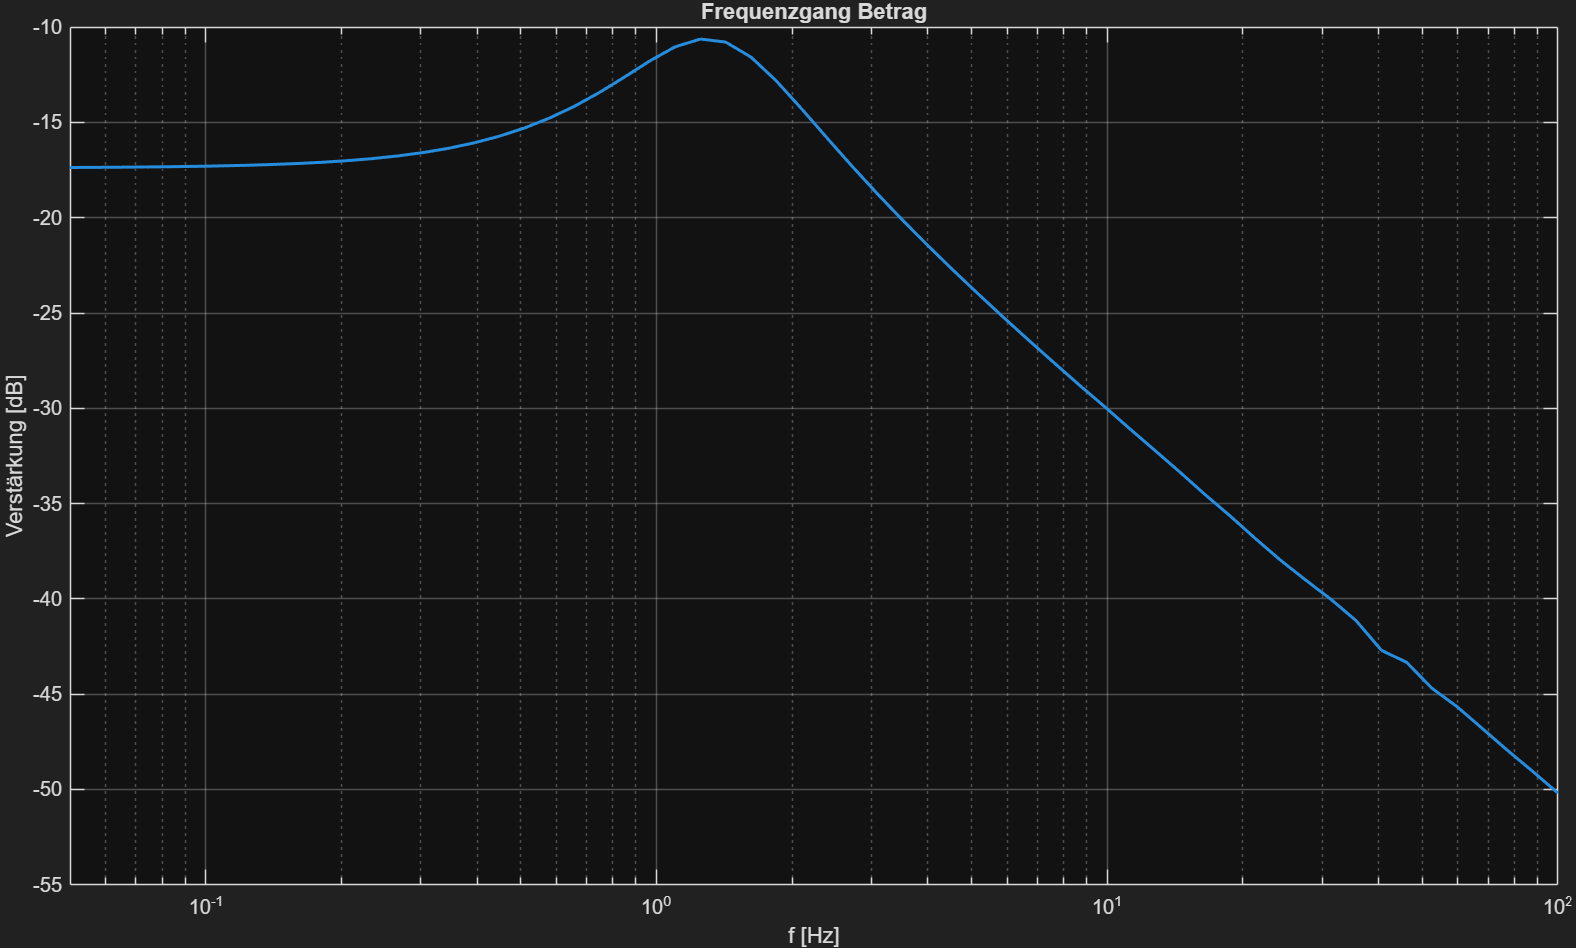
\includegraphics[width=0.95\linewidth]{pictures/Aufgabe4Amplitude.png}
    \caption{Amplitudengang des Schwimmwinkel $\beta$ bei Verwendung des nichtlinearen Einspurmodells bei einem Lenkwinkelsprung auf $1^\circ$.}
    \label{fig:aufgabe4amplitude}
\end{figure}

\begin{figure}[h]
    \centering
    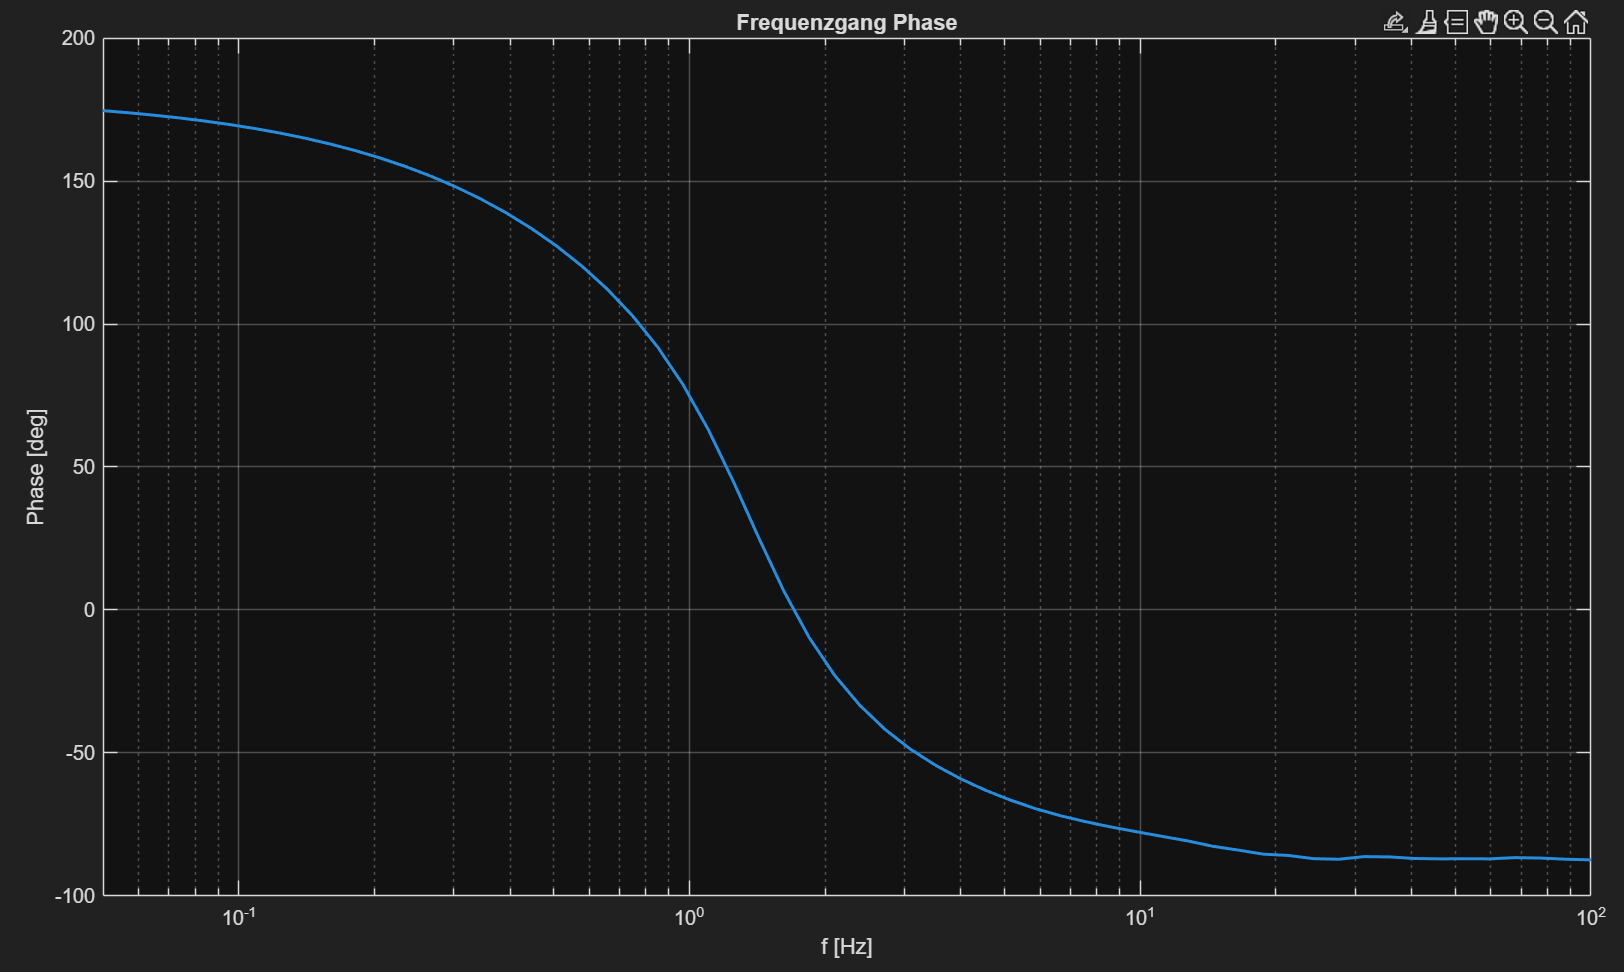
\includegraphics[width=0.95\linewidth]{pictures/Aufgabe4Phase.png}
    \caption{Phasengang des Schwimmwinkel $\beta$ bei Verwendung des nichtlinearen Einspurmodells bei einem Lenkwinkelsprung auf $1^\circ$.}
    \label{fig:aufgabe4phase}
\end{figure}

\subsection{Interpretation}
Die Abbildungen~\ref{fig:aufgabe4amplitude} und~\ref{fig:aufgabe4phase} zeigen den Amplituden- und Phasengang der \"Ubertragungsfunktion von $\delta$ nach $\beta$.
Bei niedrigen Frequenzen ist der Amplitudengang nahezu konstant (ca. $-17\,\mathrm{dB}$), d.\,h.\ langsame Lenkbewegungen
werden vom Fahrzeug quasi-station\"ar nachgebildet und der Schwimmwinkel bleibt im Verh\"altnis zur Lenkanregung klein.
Ein Wert von $-17\,\mathrm{dB}$ entspricht einem Amplitudenverh\"altnis von ungef\"ahr
$|G|\approx 10^{-17/20}\approx 0{,}14$, sodass bei einer Sinusanregung mit $\hat{\delta}=1^\circ$ eine
Schwimmwinkelamplitude von etwa $\hat{\beta}\approx 0{,}14^\circ$ zu erwarten ist.

Im Bereich um $\omega \approx 8$--$10\,\mathrm{rad/s}$ ist eine \"Uberh\"ohung (Peak) erkennbar (ca. $-10\,\mathrm{dB}$).
Dies deutet auf ein unterd\"ampftes Eigenverhalten des Systems hin: Bei Anregung nahe dieser charakteristischen Frequenz
reagiert der Schwimmwinkel \"uberproportional, was im Zeitbereich typischerweise mit \"Uberschwingen bzw. ged\"ampften
Schwingungen einhergeht. Oberhalb dieses Bereichs f\"allt der Amplitudengang stark ab, was einem Tiefpassverhalten entspricht:
Schnelle Lenkanregungen werden aufgrund von Tr\"agheit und Dynamik des Fahrzeugs nur noch stark abgeschw\"acht in $\beta$
abgebildet.

Der Phasengang startet bei niedrigen Frequenzen nahe $180^\circ$ (entspricht einer Vorzeichenumkehr in der gew\"ahlten
Signaldefinition) und dreht im \"Ubergangsbereich stark ab. F\"ur hohe Frequenzen n\"ahert sich die Phase etwa $-90^\circ$,
was ein deutlich verz\"ogertes Folgeverhalten des Schwimmwinkels gegen\"uber der Lenkanregung beschreibt:
Bei schnellen Lenkoszillationen kann das System nicht mehr unmittelbar folgen, sondern reagiert zunehmend phasenverschoben.
    \newpage
    \section{Aufgabe 5}
    
\subsection{Laden vom Simulink Modell}

Damit wir mit dem Simulink Modell arbeiten können, muss dies zunächst in das Matlab Skript eingebunden werden. 
Hierfür wird die Simulink Funktion load\_model verwendet, um das Simulink Modell in den Matlab Arbeitsbereich zu laden. 
Anschließend können die Eingänge des Modells mit der Funktion set\_param angepasst werden, um die gewünschte Geschwindigkeit zu simulieren.
Die Simulation wird für verschiedene Geschwindigkeiten durchgeführt, und der stationäre Schwimmwinkel wird für jede Geschwindigkeit berechnet.
Somit können wir die Schwimmwinkelwerte für die verschiedenen Geschwindigkeiten vergleichen und die optimale Geschwindigkeit bestimmen, bei der der stationäre Schwimmwinkel minimal ist.

\subsection{stationäre Schwimmwinkel in eingeschwungenen Zustand}
Die Simulationsergebnisse liefern uns die Time Series Daten für den Schwimmwinkel über die Zeit. Um den stationären Schwimmwinkel $\beta_{ss} = \lim_{t \to \infty} \beta(t)$ im eingeschwungenen Zustand zu bestimmen, betrachten
wir den Mittelwert des Schwimmwinkels in der letzten Sekunde der Simulation. Dieser Mittelwert dient als Näherung für den stationären Schwimmwinkel, 
da sich das System in diesem Zeitraum bereits eingependelt hat und die transienten Effekte weitgehend abgeklungen sind.

Für die Optimierung der Geschwindigkeit simulieren wir das Einspurmodell für verschiedene Geschwindigkeiten und berechnen jeweils den stationären Schwimmwinkel, damit definieren wir eine Funktion 
$\beta_{ss}(v)$, die den stationären Schwimmwinkel in Abhängigkeit von der Geschwindigkeit $v$ angibt.

\subsection{Optimale Geschwindigkeit}
Die optimale Geschwindigkeit wird durch die Minimierung des Betrags des stationären Schwimmwinkels $\beta_{ss}(v)$ bestimmt. Hierfür verwenden wir die Funktion \emph{fminbnd}, die eine eindimensionale Funktion minimiert.
Die Funktion fminbnd benötigt als Eingabe eine Funktion, die in einem gegebenen Intervall minimiert werden soll. In unserem Fall ist die Funktion, die minimiert werden soll, der Betrag des stationären Schwimmwinkels $\beta_{ss}(v)^2$ 
und das Intervall für die Geschwindigkeit $v$ wird entsprechend der realistischen Fahrgeschwindigkeiten festgelegt, z.B. von 0 bis 200 km/h.

\newpage
\subsection{Güte Funktion}
Wie schon in vorherigen Abschnitt beschrieben, minimiert die Funktion \emph{fminbnd} den Betrag des stationären Schwimmwinkels. Das ist eine Art 
Nullstellenbestimmung, da wir die Geschwindigkeit suchen, bei der der stationäre Schwimmwinkel möglichst nahe bei Null liegt.

\begin{equation*}
    v_{opt} = \arg\min_{v} |\beta_{ss}(v)|
\end{equation*}

für 

\begin{equation*}
    \beta_{ss}(v) \rightarrow^{v \to v_{opt}} 0
\end{equation*}


Da fminbnd keine Nullstellen, sondern Minima auf einem Intervall bestimmt, wird das Problem in ein Minimierungsproblem überführt. Dazu definieren wir eine nichtnegative Zielfunktion, eine Gütefunktion $\phi(v)$
\begin{equation*}
    \phi(x) := g(x)^2
\end{equation*}

Dann gilt:
\begin{equation*}
    \phi(x) \geq 0 \quad \forall x
\end{equation*}
\begin{equation*}
    \phi(x) = 0 \Leftrightarrow g(x) = 0
\end{equation*}

Damit ist jede Nullstelle von $g$ eine globale Minimierungsstelle von $\phi$ mit Minimalwert 0.
Also kann man die Nullstellenbestimmung als
\begin{equation*}
    \arg\min_{x} \phi(x) = \arg\min_{x} g(x)^2
\end{equation*}
formulieren, was mit \emph{fminbnd} gelöst werden kann.

\newpage

\subsection{Optimale Geschwindigkeit und Interpretation des Fahrverhaltens}

Die Optimale Geschwindigkeit $v_{opt}$, bei der der stationäre Schwimmwinkel minimal ist, wurde durch die Anwendung der Funktion \emph{fminbnd} auf die Funktion $\beta_{ss}(v)^2$ bestimmt. 
mit: 
\begin{equation*}
    v_{opt} = 13,93 \mathrm{m/s} \approx 50,15 \mathrm{km/h}
\end{equation*}

und dem entsprechenden stationären Schwimmwinkel von:
\begin{equation*}
    \beta_{ss}(v_{opt}) \approx 0 
\end{equation*}

\begin{figure}[H]
    \centering
    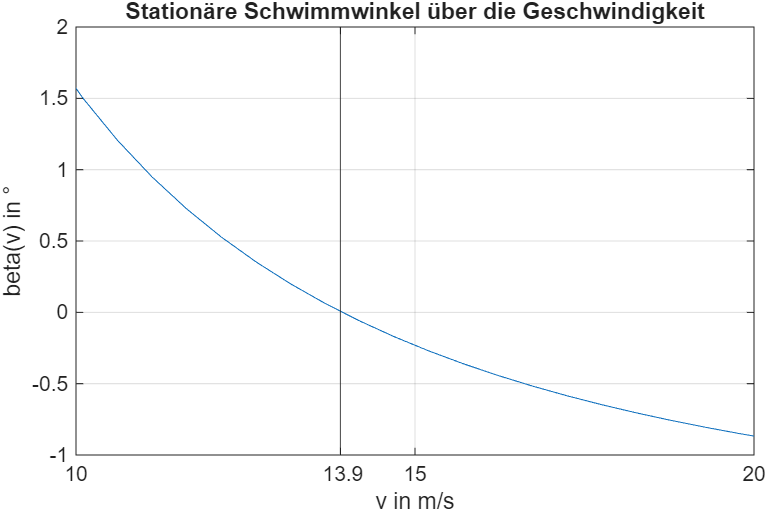
\includegraphics[width=0.75\linewidth]{pictures/ss_beta_ueber_v .png}
    \caption{Entwicklung des stationären Schwimmwinkels $\beta_{ss}$ über die Geschwindigkeit $v$.}
    \label{fig:schraeglaufwinkelVerlauf}

\end{figure}

Abbildung~\ref{fig:schraeglaufwinkelVerlauf} zeigt die Entwicklung des stationären Schwimmwinkels $\beta_{ss}$ über die Geschwindigkeit $v$ 
und dass bei der optimalen Geschwindigkeit von etwa 50 km/h der stationäre Schwimmwinkel nahezu null ist, was auf eine stabile Fahrdynamik hinweist,
bedeutet, dass der richtung der Fahrzeugbewegung $\delta$ bei der Geschwindigkeit mit der Fahrzeuglängsrichtung $v_s$ übereinstimmt. 
Bei niedereren Geschwindigkeiten hat der Schwimmwinkel einen positiven Wert, was darauf hindeutet, dass 
die Fahrzeugbewegung links von der Richtung der Fahrzeuglängsrichtung abweicht
und bei höheren Geschwindigkeiten hat der Schwimmwinkel einen negativen Wert, was darauf hindeutet, dass die Fahrzeugbewegung rechts von der Richtung der Fahrzeuglängsrichtung abweicht.


\begin{figure}[H]
    \centering
    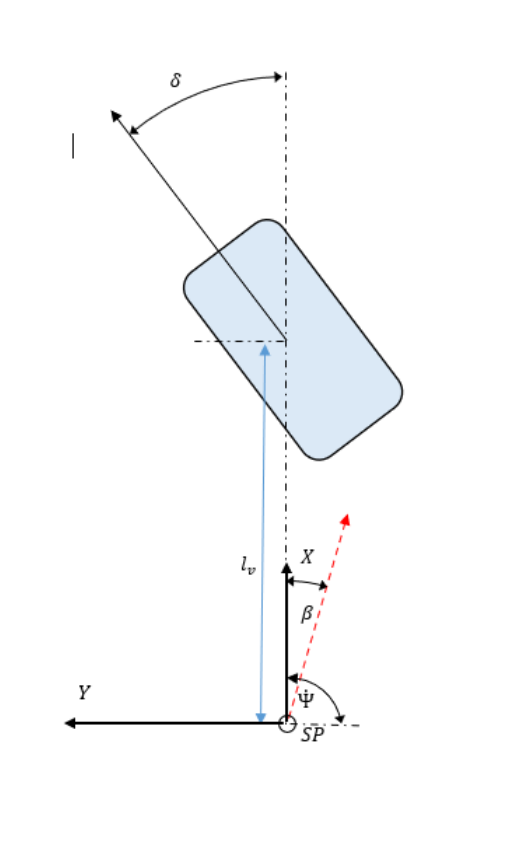
\includegraphics[width=0.5\linewidth]{pictures/schwimm.png}
    \caption{Darstellung des Schwimmwinkels im Einspurmodell.}
    \label{fig:schwimmmwinkel}

\end{figure}

Anmerkung: Der rote gestrichelte Pfeil in Abbildung~\ref{fig:schwimmmwinkel} zeigt die Richtung der Fahrzeugbewegung $v_s$, die durch den Schwimmwinkel $\beta$ von der Fahrzeuglängsrichtung $v$ abweicht.



\end{document}